\documentclass[12pt]{article}
\usepackage{geometry}
\geometry{left=2cm,right=2cm,top=2.8cm,bottom=2cm}
\setlength{\headheight}{18pt}
\setlength{\headsep}{18pt}
\setlength{\footskip}{25pt}


%\usepackage{mathptmx}
\usepackage{newtxtext}
%\usepackage{fontspec}
%\setmainfont{Times New Roman}

\usepackage{tocloft}
\usepackage{hyperref}
\usepackage{amsmath,amssymb,amsthm}
\usepackage{parskip}
\usepackage{lipsum}
\usepackage{booktabs}
\usepackage{float}

%\usepackage[pdftex]{graphicx}
\usepackage{graphicx}
\usepackage{xcolor}
\usepackage{tabularx}
\usepackage{booktabs}
\usepackage{array}
\usepackage{makecell}
\usepackage{fancyhdr}
\usepackage{url}
\lhead{Team}
\rhead{}

% setting of table of contents
\renewcommand\cftsecaftersnum{.}
\renewcommand\cftsubsecaftersnum{.}
\renewcommand\cftsubsubsecaftersnum{.}

% setup hyperlink
\hypersetup{
  colorlinks=true,
  linkcolor=black,
  citecolor=blue,
  filecolor=blue,
  urlcolor=blue
}

% graphic path
\graphicspath{{./figures/}}
\DeclareGraphicsExtensions{.pdf, .jpg, .tif, .png}

% package for section etc.
\usepackage{titlesec}
\titleformat{\section}{\Large\bfseries}{\thesection.}{1.2ex}{}
\titleformat{\subsection}{\large\bfseries}{\thesubsection.}{1.2ex}{}
\titleformat{\subsubsection}{\normalfont\itshape}{\normalfont\thesubsubsection.}{1.2ex}{}

% command for line spacing
%\renewcommand{\baselinestretch}{1.1}

\setlength{\parskip}{1em}

\newtheorem{theorem}{Theorem}
\newtheorem{corollary}[theorem]{Corollary}
\newtheorem{lemma}[theorem]{Lemma}
\newtheorem{definition}{Definition}

%%%%%%%%%%%%%%%%%%%%%%%%%%%%%%%%
\begin{document}

\thispagestyle{empty}

\medskip
\begin{center}
\large\bfseries Urban Public Transport Roadmap Planning Based on Benefit Analysis
\end{center}
The popularity of electric buses represents the possibility of further progress towards the goal of sustainable development of 
urban transportation. This paper collected the city characteristic data of St. Louis, established carbon emission model, atmosphere 
model, life cycle cost model, cost-benefit model and comprehensive evaluation model, introduced linear programming, analytic hierarchy 
process and other methods, comprehensively analyzed the ecological and economic benefits of electric buses, and helped the city plan 
the update roadmap of electric buses, which has strong practical significance.

For problem 1, we need to analyze the ecological benefits that electric bus fleets can bring. From a practical point of 
view, electric buses use electric energy as a power source, and the operation process has the environmental protection characteristics 
of zero emission of pollutants. We determined that the object of the study is the most important factor affecting the ecological 
environment emitted by diesel vehicles, namely carbon dioxide. Carbon emission model was established, performance data of electric 
bus and diesel bus were collected, linear analysis method was introduced to calculate the total annual carbon emission of each bus, 
and benefit analysis was conducted by comparing the data of the two. Secondly, considering that the damage of diesel vehicles to the 
ecological environment is partly due to the emission of air pollutants, we established an atmospheric model and calculated the total 
emissions of different types of air pollutants of the two types of buses in the service life, and drew a conclusion from the analysis.

For problem 2, what we need to analyze is the financial cost-benefit problem. From the current industry development point of view, 
the operating costs of electric buses are decreasing, which is reflected in the reduction of battery prices and the continuous 
investment of government financial subsidies, which is cost-effective. Therefore, we first established the life cycle cost model, 
divided the cost generated in the life cycle of the two types of buses into two types, and analyzed and compared the cost difference 
between the two. Secondly, a cost-benefit model is established to analyze the benefits of the electric bus fleet and calculate its 
total upfront investment cost. The net present value income analysis method is introduced to calculate the net present value income 
that can be produced during the service life cycle of electric buses, and the economic benefits of electric bus operation are analyzed 
from the data.

For problem 3, we need to create a 10-year roadmap to help St. Louis plan the renewal of its electric bus fleet. 
After analysis, we divide the project cycle into four parts. During the initial assessment and planning period, we conduct market 
research and infrastructure evaluation and identify government financial subsidy options. In the pilot stage, a small number of 
electric buses are put into pilot use on selected routes, and the operation data of electric buses and passenger feedback are 
collected, so as to determine the detailed operation plan. In the phased deployment phase, the main problem is to solve the 
infrastructure problem and optimize the route. In the comprehensive transformation phase, the entire bus fleet will be electrified 
and a long-term vehicle maintenance update mechanism and a regular fleet evaluation mechanism will be established. Therefore, 
we establish a comprehensive evaluation model, introduce linear programming analysis method, determine the weight of factors 
affecting route planning, and combine the actual data to determine the optimal deployment route of electric buses.


%关键词
\vspace{0.4cm}
\noindent \textbf{Keywords: }\LaTeX,~  Roadmap,~ Benefit Analysis

\newpage
\tableofcontents
\thispagestyle{empty}
\newpage

%正文部分
\pagestyle{fancy}
\rhead{Page \thepage~of~19}
\setcounter{page}{1}
\section{Introduction}
\subsection{Restatement of the Problem}
With the continuous deterioration of the ecological environment, more and more people are aware of the importance of environmental 
protection and practice environmental protection in all aspects of life, and public transportation has become the choice of more 
and more people. At present, most buses still use diesel as a power source, but some cities have put electric buses into operation, 
which has a huge boost to energy conservation, emission reduction and pollution reduction. More and more countries and regions are 
aware of the superiority of electric buses, and are adopting policies to vigorously support the development of electric bus industry.

However, challenges include high initial costs, charging infrastructure development,lengthy charging times, and potential range 
limitations.

Based on this situation, we need to solve the following problems:

\textbullet{Construct a model to aid cities in understanding the ecological consequences of transitioning to an all-electric bus fleet.}

\textbullet{Construct a model that focuses on the financial implications associated with a conversion to e-buses.}

\textbullet{Transportation officials in metropolitan areas are exploring approaches in which they
gradually change their fleet from combustion engines buses to electric. Assuming the goal
is to have a fully electric fleet no later than 2033, utilize your previously developed
models to craft a 10-year roadmap that urban transport authorities can leverage to plan
their e-bus fleet updates.}

\textbullet{Write a one-page letter to the transportation officials of one of your chosen
metropolitan areas in which you detail your recommendation for their transition to
e-buses.}

\subsection{Overview of Our Work} %问题分析

\subsubsection{Problem 1:Ecological Benefits Analysis}
This question mainly studies the ecological benefits brought by electric buses. After analysis, we decided to directly reflect the 
impact of electric buses and diesel vehicles on the ecological environment through detailed data and then compare the ecological 
benefits brought by electric buses. First of all, considering that the main substance emitted by bus operation is carbon dioxide, 
we establish a carbon emission model, analyze the carbon emission size of the two types of vehicles combined with the collected 
performance data, and compare the results. Secondly, considering the impact of global warming, cars will also cause air pollution. 
Therefore, we established an atmospheric model to collect pollutant emission factors of other harmful substances in the two types of 
cars except carbon dioxide, and then calculated the emissions of different kinds of pollutants during the operation of the two types 
of buses, and finally conducted data analysis and comparison.

\subsubsection{Problem 2:Cost-effectiveness Analysis}
The purpose of this question is to find out whether electric buses are competitive in the market compared with diesel buses in terms 
of both costs and benefits, that is, to analyze whether the economic benefits of electric buses are worthy of large-scale use by the 
local government. First of all, considering that both electric buses and diesel buses have service life, and the process of replacing
diesel buses with electric buses is gradual, we established a life cycle cost model, determined the life cycle length as the service 
life of buses, and roughly divided the cost into acquisition cost and maintenance cost within the life cycle. Combined with the 
collected performance parameters of the two types of vehicles and the relevant city characteristics data of St. Louis, the various 
costs generated during the life cycle of the two types of vehicles were simply summed up and compared, and the market competitiveness 
of the two types of buses was compared. Secondly, the cost-benefit analysis model is established, the net present value calculation 
formula is introduced, the income is converted into data, and the economic benefit of electric buses is judged by judging the size of 
the data.

\subsubsection{Problem 3:Optimal Roadmap Planning}
This question requires us to develop a 10-year roadmap for the city's transportation authorities to help them update the city's 
electric bus fleet. First of all, we make it clear that due to the characteristics of electric buses themselves, problems such as 
infrastructure, public acceptance, and available funds need to be solved before they are put into trial use, and the completion of 
the all-electric bus fleet needs to be carried out gradually from the pilot stage where a small number of buses are put into use. 
Therefore, we will divide the 10-year renewal cycle into four stages, and will complete the renewal and mature use of the all-electric 
bus fleet at the end of these four stages. We establish a comprehensive evaluation model, enumerates multiple factors affecting route 
planning, and introduces analytic hierarchy process (AHP) to confirm the respective weights of the influencing factors, so as to 
achieve the goal of maximum passenger flow coverage and minimum operating cost in the roadmap planning.


\section{Assumptions and Justifications}
We make the following assumptions to help us with our modeling. These assumptions form the background for our subsequent analysis.

\textbullet{\bfseries{Assumption 1:the bus will run normally, independent of personal factors such as the driver and other small 
probability events such as extreme weather.}}This is because we need ensure that the many factors in the model such as service 
frequency, emissions, etc., do not produce abnormal extreme values.

\textbullet{\bfseries{Assumption 2:the investment plan of electric buses is not affected by external factors and is continuously 
supported by policies.}}This is done to ensure that the model is built according to the established plan.

\textbullet{\bfseries{Assumption 3:the purchase and maintenance cost of buses changes according to the constant annual growth rate.}}

\textbullet{\bfseries{Assumption 4:the electric bus does not have a small probability event such as a car accident and other abnormal 
circumstances in 10 years, resulting in the change of the given number and revenue cost.}}This is to reduce the impact of small 
probability events on the model.

\section{Notations}
\begin{table}[!htbp]
	\centering
		\begin{tabular}{cc}
			\toprule
			Symbol & Definition \\
			\midrule
			${ER}$ & emission reduction\\
			${CEE}$ & $C_{\text{$Emission_{\text{ebus}}$}}$ \\
			${CEDD}$ & $C_{\text{$Emission_{\text{diesel}}$}}$ \\
			${CPEE}$ & $C_{\text{$Pollutant Emission_{\text{ebus}}$}}$ \\
			${CPED}$ & $C_{\text{$Pollutant Emission_{\text{diesel}}$}}$ \\
			${NPVE}$ & $NPV_{\text{ebus}}$ \\
			${NPVD}$ & $NPV_{\text{diesel}}$ \\
			${LCC}$ & Life cycle costing \\
			${R_i}$ & Rating \\
			\bottomrule
		\end{tabular}
\end{table}

\section{Problem 1:Ecological Benefits Analysis}
\subsection{Comparison of Carbon Emission Based on Carbon Emission Model}
\subsubsection{Establishment of Model}
\subsubsection{Data Analysis}
\begin{table}[!htbp]
	\centering
	\caption{Carbon emissions influence factor table}
	\begin{tabular}{|c|c|c|c|c|}
	\hline
	  &\textbf{amount} & \textbf{annual mileage} &\textbf{Average energy consumption}&\textbf{emission factor}\\
	\hline
	\textbf{ebus} & 500 & 30000miles&1.3kwh/mile&0.75 pounds $CO_\text{2}$e/kWh\\
	\hline
	\textbf{diesel bus} &500&30000miles&0.2gallon/mile&22.38 pounds $CO_\text{2}$e/kWh\\
	\hline
	\end{tabular}
\end{table}

\begin{figure}[H]
	\centering
	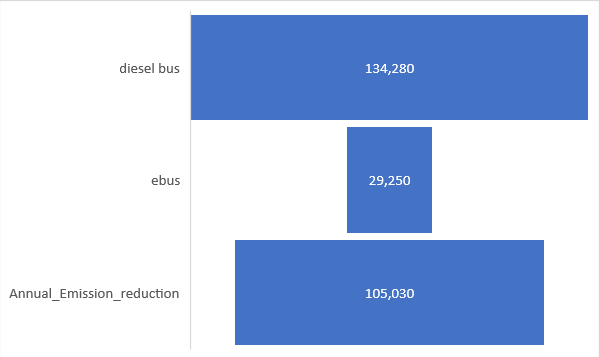
\includegraphics[scale=0.7]{Bar chart.png}% 图片相对位置
	\caption{Carbon emission comparison chart} % 图片标题
\end{figure}


\subsection{Comparison of Pollutant Emissions Based on Atmospheric Model}
\subsubsection{Establishment of Model}
\subsubsection{Data Analysis}

\section{Problem 2:Cost-effectiveness Analysis}
Life cycle cost refers to the total sum of all expenses associated with a product, service, or project throughout its entire 
lifecycle, including costs incurred during the design, development, production, operation, maintenance, and disposal phases. 
Calculating the life cycle cost helps in a more comprehensive evaluation and management of the economic benefits and feasibility 
of a project or product. To explore the economic benefits and feasibility of the electric bus deployment plan, this study sequentially 
establishes life cycle cost model and cost-benefit analysis model to analyze the market cost competitiveness and economic benefits 
of electric buses.
\subsection{Cost Comparison Based on Life Cycle Costing Model}
\subsubsection{Establishment of Model}
Based on the life cycle theory, this paper establishes the life cycle cost analysis model of electric bus and diesel vehicle, 
and accounts the total cost of the two kinds of buses during the life cycle.
First of all, the life cycle cost components of the two types of buses should be clarified. According to the life cycle stage 
of the bus, the whole life cycle cost is divided into two parts: acquisition cost and operation and maintenance cost.

\textbullet{Acquisition Cost}

In the electric bus investment plan, we need to take into account the total acquisition cost of electric buses in 10 years. 
In general, the acquisition cost is the cost of only purchasing buses in the initial stage of project construction, which is usually 
reflected in the product of the total number of vehicles purchased and the unit price of vehicles purchased. Then we get the formula 
for calculating the total acquisition cost $TC_{acquisition}$ as follows:
\begin{equation}
    TC_{\text{acquisition}} = N \cdot C_{\text{initial}}
\end{equation}
Where, $N$ represents the total number of vehicles purchased and $C_{initial}$ represents the initial purchase cost of each vehicle.

\textbullet{Operation and maintenance cost}

In the process of formally implementing the 10-year investment plan, the operation and maintenance cost of electric buses can not be ignored. Operation and maintenance cost refers to the cost incurred during the operation and maintenance of buses, which is embodied in the electricity cost generated by the operation of electric buses after a distance, the fuel cost generated by the operation of diesel buses after a distance, and the cost incurred during the annual vehicle maintenance and maintenance of the two types of vehicles.
The total operating cost $TC_{operation}$ of the bus is calculated as follows:
\begin{equation}
    TC_{\text{operation}} = N \cdot D \cdot C_{\text{operation}} 
\end{equation}
Among them, the average annual driving distance of each bus is $D$, and the average electricity or fuel cost generated by 
each bus during operation is $C_{operation}$.

The calculation formula of bus total maintenance cost $TC_{maintenance}$ is as follows:
\begin{equation}
    TC_{\text{maintenance}} = L \cdot N \cdot C_{\text{maintenance}} 
\end{equation}
Among them, the average annual maintenance cost of the bus is $C_{maintenance}$, and the expected service life of the bus is $L$.

The Operation and maintenance cost is the sum of total operation cost $TC_{operation}$ and total maintenance cost $TC_{maintenance}$.

\textbullet{Salvage value}
In the process of officially implementing the 10-year investment plan, electric public vehicles will also have problems such as 
failure and cannot continue to operate. Because the buses that exceed the expected service life are no longer involved in the operation 
of urban bus lines, in order to maximize the benefits, the scrapped buses are usually sold to extract the residual value of the buses 
and save investment costs. Therefore, the total life cycle cost should also consider the impact of the residual value of the bus after 
scrapping. Assuming that the residual value of the bus after scrapping is $Residual_{value}$, the calculation formula of residual value 
$Residual_{value}$ is as follows:

\begin{equation}
    Residual_{\text{value}}=C_{\text{initial}} \cdot \left(1-\frac{l}{L}\right)
\end{equation}
Where $l$ is the number of years used and $L$ is the expected service life of the bus.

The formula for calculating the total residual value is as follows:
\begin{equation}
    Total_{\text{Residual}_{\text{value}}}=N \cdot Residual_{\text{value}}
\end{equation}
\textbullet{In summary, we give the calculation formula of the whole life cycle cost $TC$:}
\begin{equation}
	TC=N \cdot C_{\text{initial}}+L \cdot N \cdot C_{\text{maintenance}}+N \cdot D \cdot C_{\text{operation}} -N \cdot Residual_{\text{value}}
\end{equation}

\subsubsection{Data Analysis}
We investigated Proterra Inc., a giant manufacturer of electric buses in the United States. The current performance parameters of 
electric buses and diesel buses, including purchase price, expected service life, energy consumption, annual mileage and other data, 
were obtained from the official website of Flyer Industries, the largest bus manufacturer in North America, and the electricity price 
and oil price in St. Louis were obtained by inquiring the United States Energy Information Administration. The relevant data table is 
summarized as follows:
\begin{table}[!htbp]
	\centering
	\caption{Bus Performance Parameters Table}
	\begin{tabular}{|c|c|c|c|c|c|}
	\hline
	  &\textbf{amount} & \textbf{annual mileage} &\textbf{acquisition cost}&\textbf{energy consumption}&\textbf{maintenance cost}\\
	\hline
	\textbf{ebus} & 500 & 30000km&\$125000&130kwh/100km& \$0.05/km\\
	\hline
	\textbf{diesel bus} & 500& 30000km&\$83333&50L/100km&\$0.1/km\\
	\hline
	\end{tabular}
\end{table}


Since we assume that each vehicle will operate normally throughout its life cycle until it exceeds its useful life, the residual 
value is by definition zero. In addition, as a project with huge social and ecological benefits, the federal government and the state 
government will adopt policy subsidies, which can cover about 50\% of the entire life cycle cost of electric buses.

We use the established life cycle cost model to calculate the cost of electric buses and diesel buses during their respective 
life cycles, and the calculation results are as follows:
\begin{table}[!htbp]
		\centering
		\caption{Cost Statement}
		\begin{tabular}{|c|c|c|c|c|c|}
		\hline
		  &\textbf{$TC_\text{acquisition}$} & \textbf{$TC_\text{operation}$} &\textbf{$TC_\text{maintenance}$}&\textbf{policy subsid}&\textbf{TC}\\
		\hline
		\textbf{ebus} &\$625000000&\$56160000&\$15000000&50\%&\$343400000\\
		\hline
		\textbf{diesel bus} &\$416666666&\$180000000&\$30000000&0&\$626666666\\
		\hline
		\end{tabular}
\end{table}


Combined with the calculation results in the above table, we carry out the following analysis.

Due to the current high production cost of long-life batteries, the purchase cost of each electric bus is higher than that of diesel 
buses when other components are the same. However, the rapid development of renewable energy technology in recent years will continue 
to reduce the cost of new energy technology products such as long-life batteries; At present, the global demand for crude oil continues 
to grow, the lack of production capacity release, resulting in high diesel prices, so in terms of operating costs, electric buses 
are better than diesel buses. At the same time, based on the composition and maintenance difficulty of the internal parts of the 
electric bus, its maintenance cost is also lower than that of the diesel bus. More importantly, the federal government and the state 
government have greatly supported the electric bus industry, and the injection of external funds has greatly reduced the life cycle 
cost of electric buses. Considering the above factors, the life cycle cost of electric buses in 10 years is less than that of diesel 
buses, which has great market cost competitiveness and economic benefits.

\subsection{Economic Benefit Analysis Based on Cost-benefit Analysis Model}
\subsubsection{Establishment of Model}
In order to determine the economic value of replacing diesel buses with electric buses and gradually building an all-electric bus 
fleet, we establish a cost-benefit analysis model to analyze the economic benefits of gradually replacing diesel buses with electric 
buses, and analyze the optimal solution of the electric bus delivery plan, so as to determine whether this plan is feasible and obtain 
the optimal delivery plan.

We use the net income analysis method to evaluate the economic benefits of the project, and we divide the unit by year as the time of 
investment. Based on the above analysis of the whole life cycle cost of the two types of vehicles, we can see that the most significant 
cost savings of electric buses compared with diesel buses lies in their fuel costs. As can be seen from the above, the fuel cost of 
each electric bus compared with diesel buses is $Fuel_{\text{savings}}$about 13,860.

At the same time, the maintenance cost of electric buses is also less than the maintenance cost of diesel buses, but due to the 
continuous update of electric bus technology, in contrast, the maintenance cost of electric buses $Ebus_{\text{maintenance}}$will 
decline year by year. Diesel bus maintenance fee $Diesel_{\text{maintenance}}$will increase. Assume that the maintenance cost of 
electric buses $Ebus_{\text{maintenance}}$decreases by 2\% annually, and the maintenance cost of diesel buses $Diesel_{\text{maintenance}}$increases by 2\% annually. We can regard the maintenance cost of the two as an equal proportion series, which is convenient for later solving.

Similarly, the construction cost and purchase of charging piles for each electric bus will also decrease year by year due to 
technological update. Assume that the construction cost of charging piles for electric buses $Construction_{\text{cost}}$will 
decrease by 4\% annually. The purchase cost of electric buses $Ebus_{\text{acquisition}}$will drop by 3\ annually, and we will 
also look at the two as an equal ratio series.

From this, we can get diesel bus maintenance cost $Diesel_{\text{maintenance}}$, electric bus maintenance 
cost $Ebus_{\text{maintenance}}$, Electric bus charging pile construction cost $Construction_{\text{cost}}$, 
electric bus acquisition cost $Ebus_{\text{acquisition}}$general expression, as follows:
\begin{equation}
    y_i=y_{i-1} \cdot (1+c)
\end{equation}
We determine the total size of the bus as $N$, and assume that we have invested $n_i$ electric buses by the first $i$year of the 
project.

To sum up, what is the benefit of our project requiring electric buses to replace diesel buses? You can do this by comparing the 
cost savings of electric buses in that year relative to diesel buses $Cost_{{\text{savings}}_{\text{i}}}$ with the acquisition cost 
already incurred in that year $Ebus_{{\text{acquisition}}_{\text{i}}}$and the charging points already generated in that year After 
deducting the construction cost $Construction_{{\text{cost}}_{\text{i}}}$, the total data generated during the ten years of the project 
can be summed to obtain the ten-year income of the project. The formula for calculating the total profit $TR$ is as follows:
\begin{equation}
    TR=\sum_{i=1}^{10} x_i[(\sum_{k=i}^{10} Fuel_{\text{savings}}+Diesel_{\text{maintenance}_{\text{k}}}-Ebus_{\text{maintenance}_{\text{k}}})-Ebus_{\text{acquisition}_{\text{i}}}-Construction_{{\text{cost}}_{\text{i}}}]
\end{equation}
\subsubsection{Data Analysis}
The collected and summarized data in problem 1 is substituted into the solution formula of total profit $TR$, and the following 
data can be obtained by running it.
\begin{figure}[H]
	\centering
	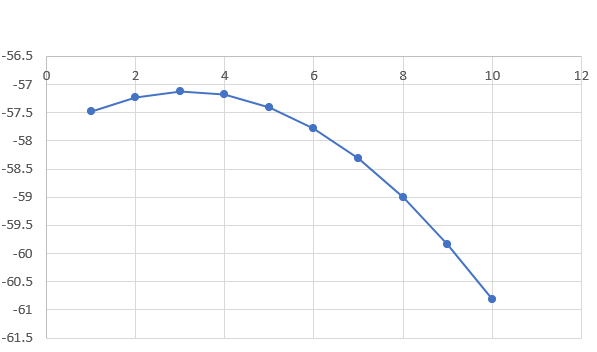
\includegraphics[scale=0.7]{data.png}% 图片相对位置
	\caption{TR Ten Year Data Analysis Chart} % 图片标题
\end{figure}
Analysis of the data shows that $TR_1>TR_2>\ldots>TR_{10}$, that is if and only if $n_1=N, n_2=n_3=\ldots= n_{10}=0$. Takes the maximum value.

As bus is a means of public transport, it usually pays more attention to social benefits. Therefore, in order to make the public 
equally enjoy the public infrastructure of bus, the government usually adopts the way of lowering the ticket price to achieve the 
inclusiveness of infrastructure. Therefore, similar to the construction of other public infrastructure, the electric bus project will 
have a period of difficulty in making ends meet after it is put into use, which is called the investment payback period in economics. 
Therefore, when we analyze programs that are in the payback period, we tend to use investment programs with fewer initial losses. 
According to the above data analysis, only when the electric bus is purchased and put into use in the first year of the project will 
the loss of the investment payback period be minimized.

In summary, although the income of electric buses in the period of investment recovery is negative, its development potential is 
huge. After determining the optimal investment plan, although it is difficult to return the cost in the short term, its economic 
income will pick up in the long run, and drive the economic development around the bus lines.

\section{Problem 3:Optimal Roadmap Planning Problems Based on Comprehensive Evaluation Model}
\subsection{Optimal Roadmap Planning Based on Comprehensive Evaluation Model}
The comprehensive evaluation model is a method to comprehensively evaluate a specific object by considering multiple indexes, 
factors or dimensions comprehensively. This model is often used in decision making, project evaluation, risk management and other 
fields. The comprehensive evaluation model considers multiple evaluation indicators, which can be qualitative or quantitative. 
This allows for a more comprehensive and objective assessment of all aspects of the object. Models often involve assigning weights 
to different indicators to reflect their relative importance in the overall evaluation. These weights can be determined based on 
expert judgment, statistical analysis, or other methods. The comprehensive evaluation model combines scores of different indicators
to generate a comprehensive score. Based on this score, objects can be ranked or classified to help make decisions.

\textbullet{\textbf{Step 1:Determine the weight}}

\textbf{Step 1.1:Establish the hierarchical structure model}

We make the problem organized and hierarchical, and construct a hierarchical structure model. These levels can be divided into 
three categories: the destination level, the middle level, and the bottom level. Among them, the number of elements of the criterion 
layer in the hierarchical structure is related to the influencing factors of the route, which are respectively: passenger flow, 
charging station location, route length, service frequency and operating cost. Ridership represents the average daily ridership of 
each route; Charging station location represents the number and location of charging stations on each route; Route length represents 
the total length of each route; Service frequency represents the bus departure interval of each route; Operating costs represent the 
expected operating costs of each route, including maintenance, energy and personnel expenses. The hierarchy is shown below:
\begin{figure}[H]
	\centering
	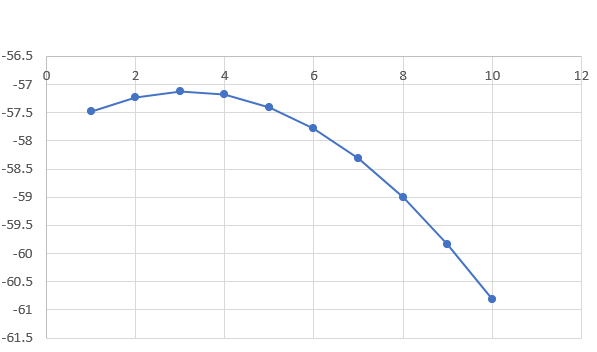
\includegraphics[scale=0.7]{data.png}% 图片相对位置
	\caption{TR Ten Year Data Analysis Chart} % 图片标题
\end{figure}

\textbf{Step 1.2:Construct judgment matrix}

The proportion of each criterion in the target measurement is not necessarily the same, and each criterion occupies a certain 
proportion. We define the judgment matrix $A= (a_{ij}) _{n \cdot n}$ by referring to the numbers $1-9$ and their reciprocal as scales.

\begin{table}[!htbp]
	\centering
	\small
	\begin{tabular}{cp{10cm}}
			\toprule
			scale & Definition \\
			\midrule
			${1}$ & Both factors are of equal importance\\
			${3}$ & Compared with the two factors, the former is slightly more important than the latter\\
			${5}$ & Compared with the two factors, the former is significantly more important than the latter\\
			${7}$ & Compared with the two factors, the former is more important than the latter\\
			${9}$ & Compared with the two factors, the former is extremely important than the latter \\
			${2,4,6,8}$ &The median value of the above adjacency judgments \\
			${reciprocal}$ &If the ratio of the importance of factor $i$ to factor $j$ is $a_{\text{ij}}$, then the ratio of the importance of factor $j$ to factor $i$ is $a_{\text{ji}}=\frac{1}{a_{i}}$ \\
			\bottomrule
	\end{tabular}
\end{table}

\textbf{Step 1.3:Single hierarchical sort and its consistency test}

Step 1.3.1:Calculate the consistency index $CI$
\begin{equation}
   CI=\frac{{\lambda_{\text{max}} - n}}{{n-1}}
\end{equation}
Step 1.3.2:Finds the consistency indicator $RI$


Step 1.3.3:Calculate the consistency ratio $CR$
\begin{equation}
	CI=\frac{CI}{RI}
 \end{equation}
 When $CR<0.10$, it is considered that the consistency of the judgment matrix is acceptable, otherwise the judgment matrix should be modified appropriately
 
 \textbf{Step 1.4:Total hierarchical ranking and its consistency Test (Eigenvector method)}

 Multiply the weight vector $W$ right by the weight matrix $A$, there is:
 \begin{equation}
	AW=\lambda_{\text{max}}W
 \end{equation}

\textbullet{\textbf{Step 2:Determine the scoring criteria}}

\textbf{Step 2.1:Passenger flow}

Use the linear transformation method. Map the ridership of each route to a fixed range (for example, 0 to 100). 
The specific calculation formula is as follows:
\begin{equation}
	P_i = \left(\frac{{R_A - R_L}}{{R_H - R_L}}\right) \cdot 100
\end{equation}
 
Where, $P_i$ is the passenger flow score of route $i$; $R_A$ is the daily average passenger flow of this route; $R_H$ is the maximum daily passenger 
 flow of the route; $R_L$ is the minimum daily ridership of the route.

\textbf{Step 2.2:Location of charging station}
The score is based on the number of charging stations on each route. The specific calculation formula is as follows:
\begin{equation}
C_i = \frac{{N_i}}{{N_{\text{max}}}} \cdot 100
\end{equation}
Where, $C_i$ is the score of the charging station location of route $i$; $N_i$ is the number of charging stations on the route; $N_{text{max}}$ is the number of charging 
stations on the route with the most charging stations of all routes.

\textbf{Step 2.3:Route length}

Consider the length of the route and the endurance of the electric bus. Using the normal distribution method, a longer route may require a higher score, 
provided the electric bus can cover that length. Only the length of a single trip is considered here. The specific calculation formula and image are as follows:
\begin{equation}
	L_i = 100 \cdot e^{\left(-\frac{{(x-20)^2}}{{98/(\ln 2)}}\right)}
\end{equation}

\begin{figure}[H]
	\centering
	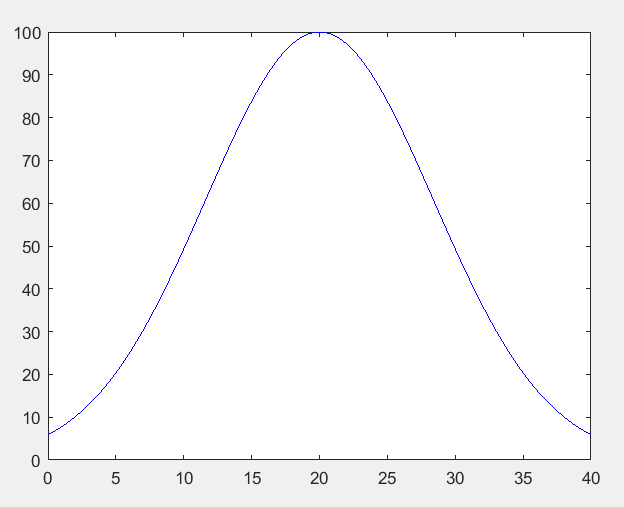
\includegraphics[scale=0.7]{data analysis.png}% 图片相对位置
	\caption{TR Ten Year Data Analysis Chart} % 图片标题
\end{figure}

Where, $L_i$ is the route length score of route $i$; $x$ is the length of route $i$. As shown in the figure, the figure shows the score obtained by the route length with 
the value range of $0-40$ km according to the rule of normal distribution. If the route length is too low, it indicates that the tram has not completed the maximum 
mileage, and the cost performance of the route is low. If the length of the route exceeds the maximum mileage, the benefit of the route is low. When the distance 
is moderate and just the mileage, the cost performance and benefit are the best, and the highest score is accordingly.

\textbf{Step 2.4:Service frequency}

Use linear conversion or categorical scoring methods. Routes with more frequent service receive higher ratings. 
The specific calculation formula is as follows:
\begin{equation}
F_i=\left\{\begin{matrix} 
	50  \qquad t=0.5h\\ 
	100 \qquad t=1h
	\end{matrix}\right.  
\end{equation}  
Among them, $F_i$ is the service frequency score of route $i$; $t$ is the service frequency for this route. After numerical preprocessing, 
we find that the service frequency is roughly one every hour and one every half hour, so the two service frequencies are assigned 100 and 50 points 
respectively.

\textbf{Step 2.5: Operating costs:}

Use the linear conversion method. Lower cost routes receive higher ratings. The specific calculation formula and image are as follows:
\begin{equation}
	O_i = \frac{214}{\pi} \cdot \arctan{\left(\frac{20-x}{2}\right)} 
\end{equation}

\begin{figure}[H]
	\centering
	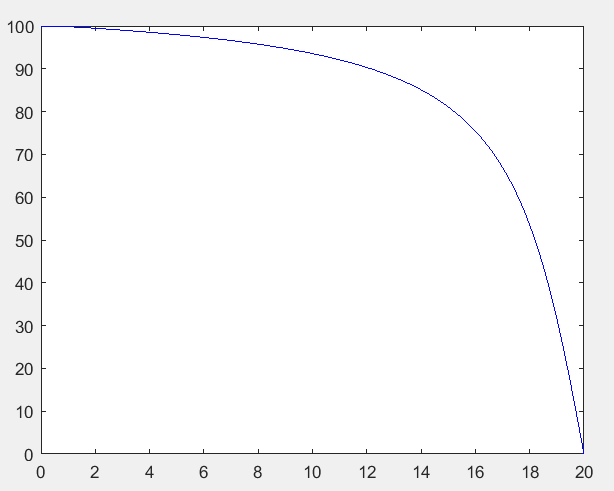
\includegraphics[scale=0.7]{data analysis1.png}% 图片相对位置
	\caption{TR Ten Year Data Analysis Chart} % 图片标题
\end{figure}
Where, $O_i$ is the operating cost score of route $i$; $x$ is the operating cost of the route. As shown in the figure, this graph represents the operating 
cost in the range of \$0 to \$20 as scored according to the law of the arc-tangent function. The lower the operating cost, the higher the score; The reverse 
is also true.

\textbullet{\textbf{Step 3:Allotment score}}

Each factor data of each route is brought into the scoring standard of each data and the corresponding score is obtained.

\textbullet{\textbf{Step 4:Comprehensive score}}

$Ri$ is set as the total score of route i, and the specific calculation formula is as follows:
\begin{equation}
	R_i = w_1 \cdot P_i + w_2 \cdot C_i + w_3 \cdot L_i + w_4 \cdot F_i + w_5 \cdot O_i 
\end{equation}
Where $P_i$ is the ridership score of Route $i$. $C_i$: Charging station location score for Route $i$. $L_i$: 
The length score of route $i$. $F_i$: Service frequency score for Route $i$. $O_i$: Operating cost score for Route $i$. $w_1,w_2,w_3,w_4,w_5$: The weights of ridership, 
charging station location, route length, service frequency, and operating cost, respectively.

\subsection{Data Analysis}
We inquired the official website of Bureau of Transportation Statistics and collected the relevant data of passenger flow, 
route length, charging station location, service frequency and operating cost. The judgment matrix A and its weight coefficient 
based on the analytic hierarchy process are shown as follows:
$W = \begin{bmatrix}  
	0.26042254 \\  
	0.06099529 \\  
	0.12457606\\  
	0.11164655 \\
	0.44235955
  \end{bmatrix} $
  
$A = \begin{bmatrix}  
	1 & 3 & 5 & 2 & \frac{1}{2} \\  
	\frac{1}{3} & 1 & \frac{1}{3} & \frac{1}{3} & \frac{1}{5} \\  
	\frac{1}{5} & 3 & 1 & 2 & \frac{1}{5} \\  
	\frac{1}{2} & 3 & \frac{1}{2} & 1 & \frac{1}{5} \\
	2 & 5 & 5 & 5 & 1 \\  
  \end{bmatrix} $
  
  $RI=1.12$

  $lambda_{max}:5.409565256771517$

  $Weights=[0.26042254 0.06099529 0.12457606 0.11164655 0.44235955]$

  $CR=0.09142081624364211$

Among them,$CR<0.1$ is obtained by calculation, indicating that the consistency of the judgment matrix is acceptable. 
In the $W$ matrix, $w_1,w_2,w_3,w_4 and w_5$ from top to bottom are respectively the weights of passenger flow, charging station location, 
route length, service frequency and operating cost.

After the above weights and the data processed by the scoring criteria are put into the comprehensive scoring formula, 
the scoring results and the routes obtained based on the scoring results are shown in the frequency distribution histogram and road map below:
\begin{figure}[H]
	\centering
	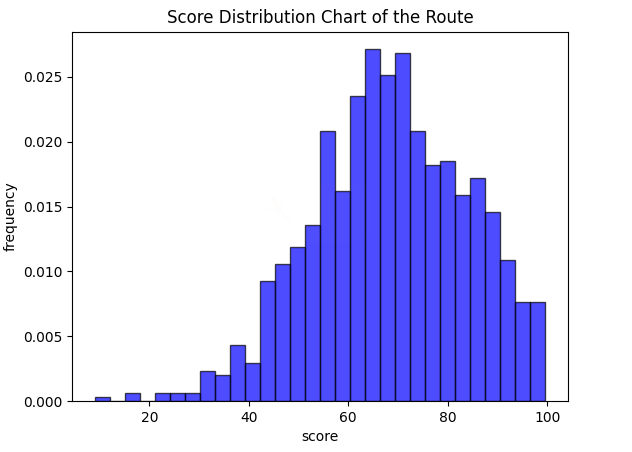
\includegraphics[scale=0.6]{score.png}% 图片相对位置
	\caption{Score distribution Chart of the Route} 
	\label{score.png}% 图片标题
\end{figure}

\begin{figure}[H]
	\centering
	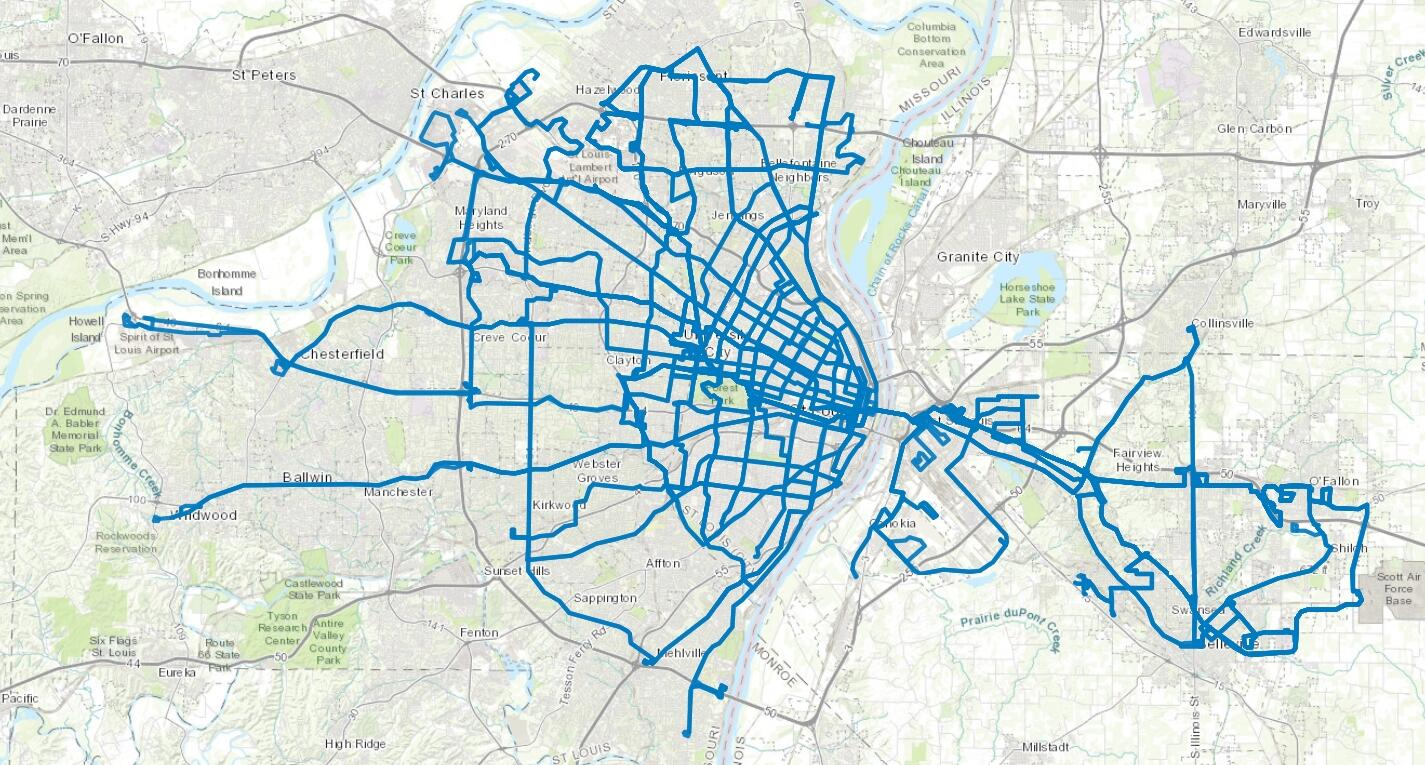
\includegraphics[scale=0.4]{city s.jpg}% 图片相对位置
	\caption{St. Louis Streetcar map} % 图片标题
	\label{city s.jpg}
\end{figure}
Among them, the route score map contains scores of many routes, so it is expressed in the form of frequency distribution 
histogram. The sample size is 1000, and the number of routes for each score is the product of the score frequency and sample size. 
The number and distribution of routes with different scores are shown in Figure \ref{score.png}. It can be found that the routes with medium 
and high scores are mostly the routes with low scores, and the routes with medium and high scores are relatively similar to the 
original bus routes. Therefore, we can make adjustments on the basis of the original bus routes, and the adjusted road map is shown 
in Figure \ref{city s.jpg}.

\subsection{Model application}
After applying the comprehensive evaluation model established above to two electric bus cities similar to St. Louis, 
Cincinnati and Houston, which are also in the initial stage, the following route scores and trolley road maps can be obtained:
\begin{figure}[htbp]
	\centering
	\begin{minipage}{0.49\linewidth}
		\centering
		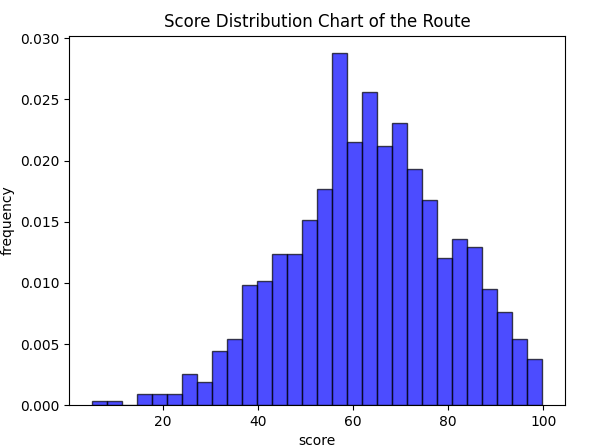
\includegraphics[width=0.9\linewidth]{score d.png}
		\caption{core distribution Chart of the Route}
		\label{score d.jpg}%文中引用该图片代号
	\end{minipage}

	\begin{minipage}{0.49\linewidth}
		\centering
		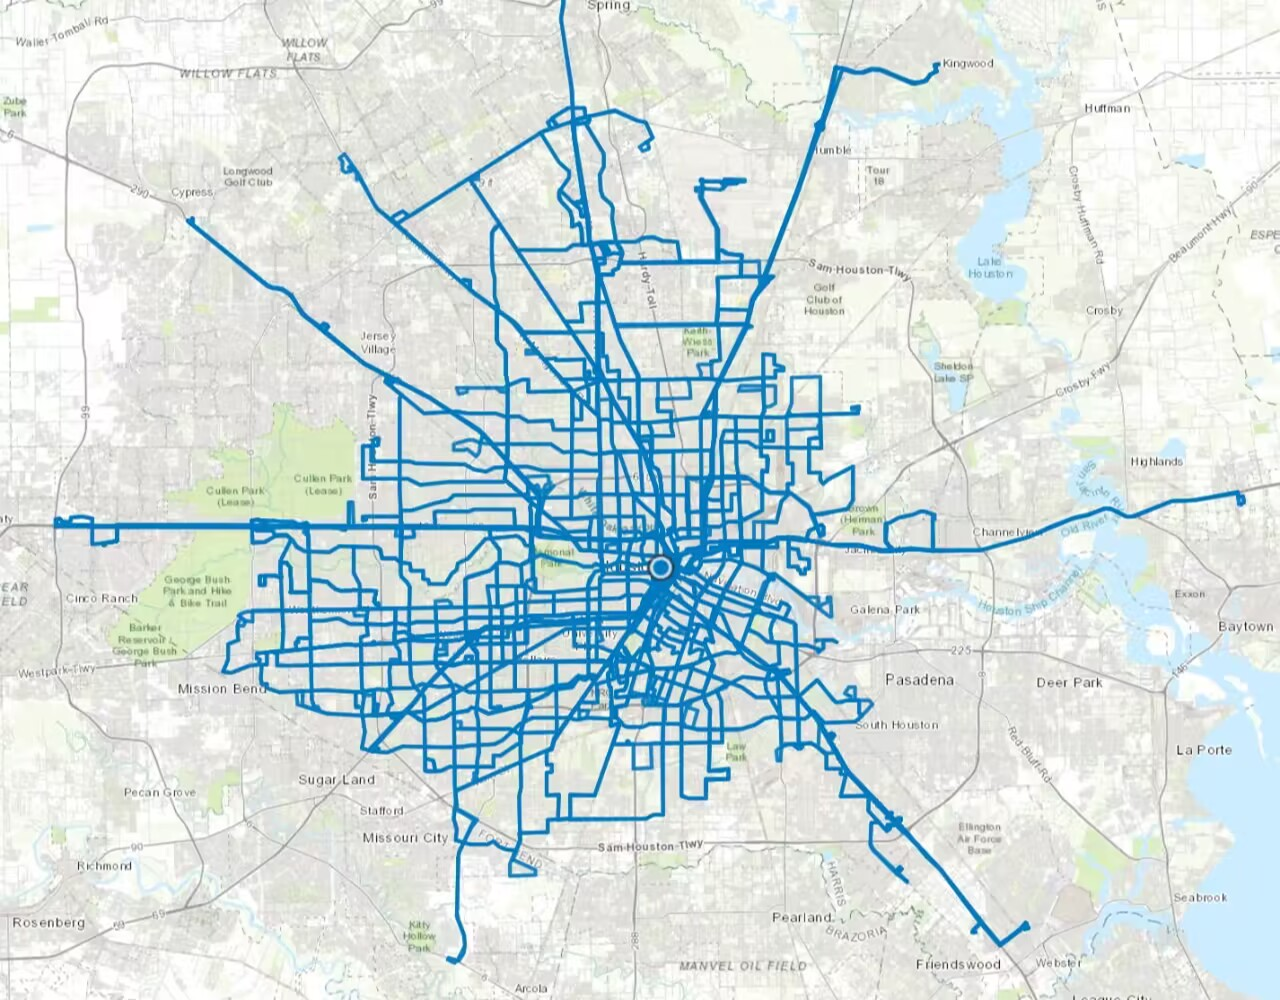
\includegraphics[width=0.9\linewidth]{city d.jpg}
		\caption{Houston Roadmap}
		\label{city d.jpg}%文中引用该图片代号
	\end{minipage}

	\qquad
	\begin{minipage}{0.49\linewidth}
		\centering
		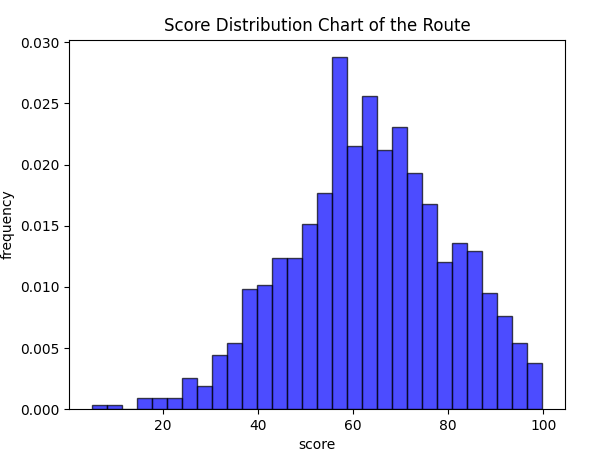
\includegraphics[width=0.9\linewidth]{score x.png}
		\caption{Score distribution Chart of the Route}
		\label{score x.jpg}%文中引用该图片代号
	\end{minipage}
\end{figure}
\newpage
\begin{figure}[htbp]
	\centering
	\begin{minipage}{0.49\linewidth}
		\centering
		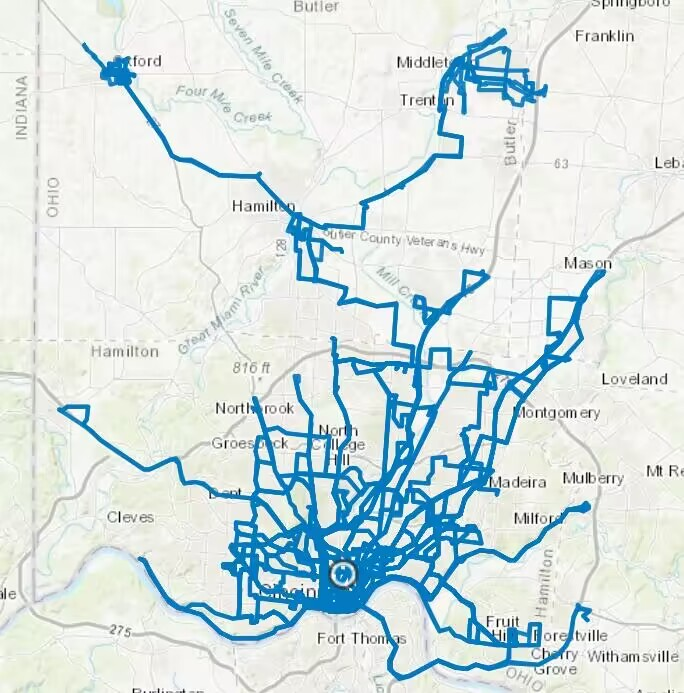
\includegraphics[width=0.9\linewidth]{city x.jpg}
		\caption{Cincinnati Road Map}
		\label{city x.jpg}%文中引用该图片代号
	\end{minipage}
\end{figure}
Among them, the analysis result of the route is roughly the same as that of St. Louis, so we can make adjustments according 
to the planning method of St. Louis, and the adjusted road map is shown in the above figure

\newpage
\section{A Letter to the Transportation Officials}
Dear Transportation Officials,

We conducted an in-depth analysis of St. Louis' public transit system, with a particular focus on the potential benefits of 
transitioning from traditional internal combustion engine buses to electric buses. The research shows that the popularization of 
electric buses will bring many advantages to St. Louis, including environmental quality improvement, economic benefit improvement, 
and significant social impact.

First, the adoption of electric buses will help improve local air quality and reduce emissions of greenhouse gases and air pollutants. 
This is essential to improve the quality of the urban environment, thereby protecting the health of citizens and enhancing the 
sustainability of cities. Our model analysis shows that the adoption of electric buses will reduce emissions of pollutants and 
greenhouse gases, contribute to the mitigation of the greenhouse effect, reduce human respiratory diseases and improve quality of life.

Second, our research finds that despite the higher initial investment cost of electric buses, the net present value benefits of 
electric buses are greater in the long run. With the continuous progress of new energy technology and the continuous improvement 
of charging infrastructure, the life cycle cost of electric buses will continue to decrease. In addition, strong policy support and 
the government's funding subsidy program will help ease the burden of initial investment.

Finally, the adoption of electric buses will help improve the local public transport system and the surrounding infrastructure 
construction, so as to beautify the city, promote technological innovation, create job opportunities, strengthen the public's 
transportation convenience, better gain the trust of the public and enhance the urban happiness index, and bring a positive impact on 
the local economic and social development.

Based on the above benefits, we strongly recommend that the transport authorities in your city consider designating a reasonable plan 
for the introduction of electric buses and develop relevant policies around this plan to ensure the smooth implementation of the plan 
and complete the transition from traditional internal combustion engine buses to electric buses. We are ready to provide further 
support, including a detailed roadmap and implementation recommendations, to help your city achieve a successful transition to electric 
buses.

On behalf of the research team, we sincerely hope that our proposal will contribute to the sustainable transportation development 
of your city. If you have any questions or need further information, we will be more than happy to assist.


\newpage

\section{Model Evaluation}
\subsection{Advantages of Model}
In analyzing the model of the city's replacement with electric buses, we adopted the method of integrating 
environmental and economic factors to ensure the comprehensiveness and practicability of the model. We considered the 
improvements in urban air quality, the reduction in energy consumption, and the long-term cost-effectiveness of electric buses.
 By simulating different scenarios, we are able to predict the effects of different policy and infrastructure changes, thus 
 providing strong support for decision makers.
\subsection{Disadvantages of Model}
However, our model is limited in some ways. First, due to the lack of detailed city-specific data, our model must rely on a number of 
assumptions and generic data, which can affect its accuracy in specific situations. Second, while we took environmental and economic 
factors into account, we failed to adequately consider social and policy factors, such as changing public acceptance of electric buses 
or uncertainty over government policy. In addition, our model does not fully consider the potential impact of technological advances 
on the performance and cost of electric buses.


\newpage
\begin{thebibliography}{100}
\bibitem{1}\url{https://afdc.energy.gov/vehicles/electric_emissions.html}
\bibitem{2}\url{https://about.bnef.com/electric-vehicle-outlook/}
\bibitem{3}\url{https://www.apta.com/research-technical-resources/transit-statistics/\\electric-bus-fact-sheets/}
\end{thebibliography}

\end{document}